\documentclass[10pt]{beamer}
\usetheme{metropolis}

% ── Packages ──
\usepackage{amsmath,amssymb,amsthm}
\usepackage{tikz}
\usetikzlibrary{positioning,arrows.meta,calc}
\usepackage{graphicx}
\usepackage{array}
\usepackage{etoolbox}

% ── Theorem environments ──
\theoremstyle{definition}
\newtheorem{defi}{Definition}[section]
\newtheorem{prop}{Proposition}[section]
\newtheorem{thm}{Theorem}[section]

% Custom theorem styles with colors
\setbeamercolor{block title}{bg=red!75!black,fg=white}
\setbeamercolor{block body}{bg=yellow!10!white}

\AtBeginEnvironment{prop}{%
  \setbeamercolor{block title}{bg=yellow!75!black,fg=black}%
  \setbeamercolor{block body}{bg=yellow!10!white}%
}
\AtEndEnvironment{prop}{%
  \setbeamercolor{block title}{bg=red!75!black,fg=white}%
}

\AtBeginEnvironment{thm}{%
  \setbeamercolor{block title}{bg=yellow!75!black,fg=black}%
  \setbeamercolor{block body}{bg=yellow!10!white}%
}
\AtEndEnvironment{thm}{%
  \setbeamercolor{block title}{bg=red!75!black,fg=white}%
}

% ── Highlighting ──
\newcommand{\x}[1]{\alert{\textbf{#1}}}
\newcommand{\rd}[1]{{\color{red!70!black}#1}}
\newcommand{\bl}[1]{{\color{blue!70!black}#1}}
\newcommand{\gn}[1]{{\color{green!60!black}#1}}
\newcommand{\ora}[1]{{\color{orange!80!black}#1}}
\newcommand{\gry}[1]{{\color{gray}#1}}

\title{Lecture 21: Positive Definite Matrices}
\subtitle{Quadratic Forms, Ellipses, and the Question $A=M^TM$}
\date{}
\titlegraphic{}

\begin{document}
\begin{frame}[plain,shrink=10]
\titlepage
\end{frame}

% ═══════════════════════════════════════
% §1 OPENING QUESTION
% ADR: Start from the factorization question A=M^T M, not from the
% definition. Students have just seen SVD and A^T A. This opening makes
% positive definiteness feel necessary: only nonnegative squared-length
% forms can come from M^T M.
% ═══════════════════════════════════════
\section{The Question}

\begin{frame}{Today's Question}

Last time, one matrix appeared again and again:

$$
M^TM.
$$

\vfill

For every vector $x$:

$$
x^TM^TMx=(Mx)^T(Mx)=\|Mx\|^2.
$$

\vfill

So $M^TM$ always produces a \x{squared length}.

\vfill

\begin{center}
{\Large \x{Which symmetric matrices can be written as $M^TM$?}}
\end{center}

\end{frame}


\begin{frame}{The Necessary Condition}

If

$$
A=M^TM,
$$

then:

$$
x^TAx=x^TM^TMx=\|Mx\|^2.
$$

\vfill

Therefore:

$$
\boxed{x^TAx\ge0\quad\text{for every }x.}
$$

\vfill

\begin{center}
\x{So a candidate $A$ must never assign negative squared length.}
\end{center}

\end{frame}


\begin{frame}{A Symmetric Matrix Measures Length?}

A real symmetric matrix $A$ gives a quadratic expression:

$$
q_A(x)=x^TAx.
$$

\vfill

If $q_A(x)$ behaves like squared length, then:

$$
q_A(x)>0\quad\text{for every }x\ne0.
$$

\vfill

If $q_A(x)$ sometimes becomes negative, it cannot be a squared length.

\vfill

\begin{center}
\x{The whole lecture is about testing this sign.}
\end{center}

\end{frame}


\begin{frame}{Look at the Unit Shape}

Instead of testing every vector one by one, draw the set:

$$
\{x:x^TAx=1\}.
$$

\vfill

This is the ``unit circle'' for the quadratic form.

\vfill

\begin{center}
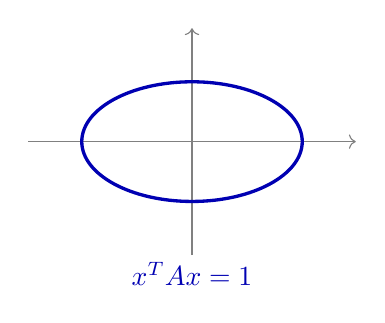
\begin{tikzpicture}[scale=0.8]
  \draw[->,gray] (-2.6,0)--(2.6,0);
  \draw[->,gray] (0,-1.8)--(0,1.8);
  \draw[blue!70!black,very thick] (0,0) ellipse (1.75 and 0.95);
  \node[blue!70!black] at (0,-2.1) {$x^TAx=1$};
\end{tikzpicture}
\end{center}

\end{frame}


\begin{frame}{If It Comes From $M^TM$}

If $A=M^TM$, then:

$$
x^TAx=1
\quad\Longleftrightarrow\quad
\|Mx\|^2=1.
$$

\vfill

So the shape is a preimage of an ordinary circle/sphere.

\vfill

\begin{center}
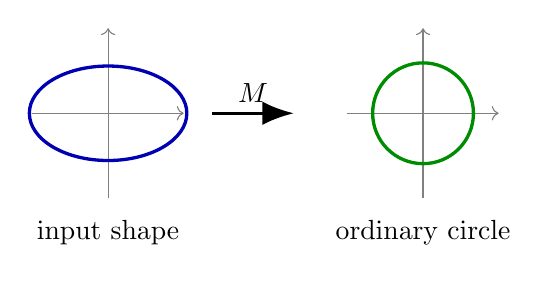
\begin{tikzpicture}[scale=0.8]
  \draw[->,gray] (-3.2,0)--(-0.8,0);
  \draw[->,gray] (-2,-1.35)--(-2,1.35);
  \draw[blue!70!black,very thick] (-2,0) ellipse (1.25 and 0.75);
  \node[below] at (-2,-1.55) {input shape};

  \draw[-{Latex[length=4mm]},very thick] (-0.35,0)--(0.95,0)
    node[midway,above] {$M$};

  \draw[->,gray] (1.8,0)--(4.2,0);
  \draw[->,gray] (3,-1.35)--(3,1.35);
  \draw[green!55!black,very thick] (3,0) circle (0.8);
  \node[below] at (3,-1.55) {ordinary circle};
\end{tikzpicture}
\end{center}

\vfill

\begin{center}
\x{This suggests ellipse-type geometry, not hyperbola geometry.}
\end{center}

\end{frame}


% ═══════════════════════════════════════
% §2 THREE SHAPES
% ADR: Give the visual evidence before definitions. The same equation
% x^T A x=1 may produce ellipse, degenerate lines, or hyperbola. These
% pictures justify why the classification is needed.
% ═══════════════════════════════════════
\section{Three Possible Shapes}

\begin{frame}{Good Case: Ellipse}

$$
A=\begin{pmatrix}\frac14&0\\0&1\end{pmatrix},
\qquad
x^TAx=1\Longleftrightarrow \frac{x^2}{4}+y^2=1.
$$

\begin{center}
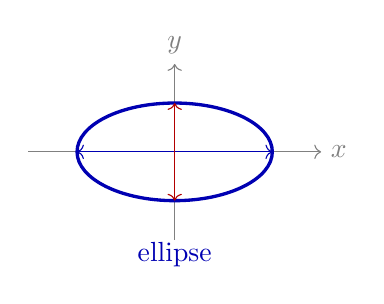
\begin{tikzpicture}[scale=0.62]
  \draw[->,gray] (-3,0)--(3,0) node[right] {$x$};
  \draw[->,gray] (0,-1.8)--(0,1.8) node[above] {$y$};
  \draw[blue!70!black,very thick] (0,0) ellipse (2 and 1);
  \draw[blue!70!black,<->] (-2,0)--(2,0);
  \draw[red!70!black,<->] (0,-1)--(0,1);
  \node[blue!70!black] at (0,-2.1) {ellipse};
\end{tikzpicture}
\end{center}

\end{frame}


\begin{frame}{Borderline Case: Two Lines}

$$
A=\begin{pmatrix}0&0\\0&1\end{pmatrix},
\qquad
x^TAx=1\Longleftrightarrow y^2=1.
$$

\begin{center}
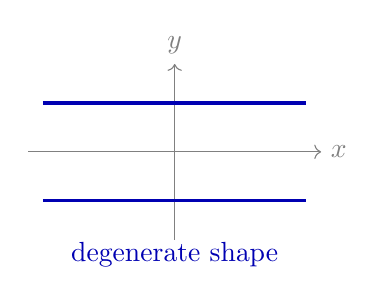
\begin{tikzpicture}[scale=0.62]
  \draw[->,gray] (-3,0)--(3,0) node[right] {$x$};
  \draw[->,gray] (0,-1.8)--(0,1.8) node[above] {$y$};
  \draw[blue!70!black,very thick] (-2.7,1)--(2.7,1);
  \draw[blue!70!black,very thick] (-2.7,-1)--(2.7,-1);
  \node[blue!70!black] at (0,-2.1) {degenerate shape};
\end{tikzpicture}
\end{center}

\begin{center}
\x{One direction has zero length.}
\end{center}

\end{frame}


\begin{frame}{Bad Case: Hyperbola}

$$
A=\begin{pmatrix}-1&0\\0&1\end{pmatrix},
\qquad
x^TAx=1\Longleftrightarrow -x^2+y^2=1.
$$

\begin{center}
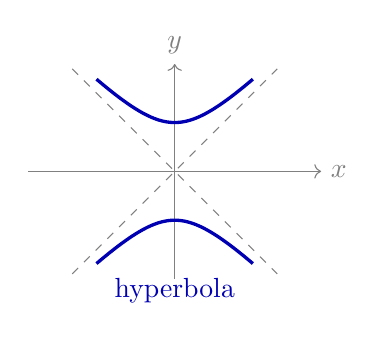
\begin{tikzpicture}[scale=0.62]
  \draw[->,gray] (-3,0)--(3,0) node[right] {$x$};
  \draw[->,gray] (0,-2.2)--(0,2.2) node[above] {$y$};
  \draw[blue!70!black,very thick,domain=-1.25:1.25,smooth,variable=\t]
    plot ({sinh(\t)}, {cosh(\t)})
    plot ({sinh(\t)}, {-cosh(\t)});
  \draw[gray,dashed] (-2.1,-2.1)--(2.1,2.1);
  \draw[gray,dashed] (-2.1,2.1)--(2.1,-2.1);
  \node[blue!70!black] at (0,-2.45) {hyperbola};
\end{tikzpicture}
\end{center}

\end{frame}


\begin{frame}{Three Shapes, Three Behaviors}

\begin{center}
\renewcommand{\arraystretch}{1.35}
\begin{tabular}{c|c|c}
\textbf{Matrix} & \textbf{Shape of $x^TAx=1$} & \textbf{Behavior}\\
\hline
$\begin{pmatrix}\frac14&0\\0&1\end{pmatrix}$ & ellipse & always positive\\
$\begin{pmatrix}0&0\\0&1\end{pmatrix}$ & two lines & never negative, but degenerate\\
$\begin{pmatrix}-1&0\\0&1\end{pmatrix}$ & hyperbola & sometimes negative
\end{tabular}
\end{center}

\vfill

\begin{center}
\x{Now we need names for these three behaviors.}
\end{center}

\end{frame}


\begin{frame}{Definitions}

\begin{defi}
Let $A$ be a real symmetric matrix.
\begin{itemize}
\item $A$ is \x{positive definite} if
$$
x^TAx>0\quad\text{for every }x\ne0.
$$
\item $A$ is \x{positive semidefinite} if
$$
x^TAx\ge0\quad\text{for every }x.
$$
\item $A$ is \x{indefinite} if $x^TAx$ takes both positive and negative values.
\end{itemize}
\end{defi}

\end{frame}


% ═══════════════════════════════════════
% §3 MATRIX AS INNER PRODUCT TABLE
% ADR: Before using e_i^T A e_i in later criteria, introduce the
% standard basis visually. The user explicitly requested a colored
% matrix picture showing how e_i selects columns/rows and diagonal
% pivots.
% ═══════════════════════════════════════
\section{Matrix as an Inner Product Table}

\begin{frame}{Where Does $x^TAx$ Come From?}

The ordinary dot product is:

$$
\langle v,w\rangle=v^Tw.
$$

\vfill

A symmetric matrix $A$ gives a new bilinear form:

$$
\boxed{\langle v,w\rangle_A=v^TAw.}
$$

\vfill

Then the quadratic form is the self-pairing:

$$
\boxed{\langle x,x\rangle_A=x^TAx.}
$$

\vfill

\begin{center}
\x{So $A$ is trying to define a new geometry.}
\end{center}

\end{frame}


\begin{frame}{Symmetry Means $A=A^T$}

For an inner-product-like geometry, we want:

$$
\langle v,w\rangle_A=\langle w,v\rangle_A.
$$

\vfill

Compute:

$$
\langle v,w\rangle_A=v^TAw.
$$

\vfill

Also:

$$
\langle w,v\rangle_A=w^TAv=(w^TAv)^T=v^TA^Tw.
$$

\vfill

So symmetry of the form is exactly:

$$
\boxed{A=A^T.}
$$

\end{frame}


\begin{frame}{Matrix Entries Are Inner Products}

\[
\scriptsize
\underbrace{
\begin{pmatrix}
a_{11}&a_{12}&a_{13}\\
a_{21}&a_{22}&a_{23}\\
a_{31}&a_{32}&a_{33}
\end{pmatrix}}_{A}
=
\underbrace{
\begin{pmatrix}
\langle e_1,e_1\rangle_A&\langle e_1,e_2\rangle_A&\langle e_1,e_3\rangle_A\\
\langle e_2,e_1\rangle_A&\langle e_2,e_2\rangle_A&\langle e_2,e_3\rangle_A\\
\langle e_3,e_1\rangle_A&\langle e_3,e_2\rangle_A&\langle e_3,e_3\rangle_A
\end{pmatrix}}_{\text{inner product table of basis vectors}}.
\]

\vfill

\[
\boxed{\underbrace{a_{ij}}_{\text{matrix entry}}
=
\underbrace{e_i^TAe_j}_{\langle e_i,e_j\rangle_A}.}
\]

\vfill

\begin{center}
\x{The matrix $A$ is the inner product table of the standard basis.}
\end{center}

\end{frame}


\begin{frame}{Standard Basis Vectors}

In $\mathbb R^3$:

$$
e_1=\begin{pmatrix}1\\0\\0\end{pmatrix},
\qquad
e_2=\begin{pmatrix}0\\\rd{1}\\0\end{pmatrix},
\qquad
e_3=\begin{pmatrix}0\\0\\1\end{pmatrix}.
$$

\vfill

The vector $e_2$ means:

\begin{center}
\x{select the second coordinate.}
\end{center}

\vfill

So multiplying by $e_2$ should select the second column or second row.

\end{frame}


\begin{frame}{Right Multiplication Selects a Column}

Let

$$
A=
\begin{pmatrix}
a_{11}&\rd{a_{12}}&a_{13}\\
a_{21}&\rd{a_{22}}&a_{23}\\
a_{31}&\rd{a_{32}}&a_{33}
\end{pmatrix},
\qquad
e_2=\begin{pmatrix}0\\\rd{1}\\0\end{pmatrix}.
$$

\vfill

Then:

$$
Ae_2=
\begin{pmatrix}
\rd{a_{12}}\\
\rd{a_{22}}\\
\rd{a_{32}}
\end{pmatrix}.
$$

\vfill

\begin{center}
\x{$Ae_2$ selects column $2$.}
\end{center}

\end{frame}


\begin{frame}{Left Multiplication Selects a Row}

Now put $e_2^T$ on the left:

$$
e_2^T=\begin{pmatrix}0&\rd{1}&0\end{pmatrix}.
$$

\vfill

Then:

$$
e_2^TA
=
\begin{pmatrix}
\rd{a_{21}}&\rd{a_{22}}&\rd{a_{23}}
\end{pmatrix}.
$$

\vfill

\begin{center}
\x{$e_2^TA$ selects row $2$.}
\end{center}

\end{frame}


\begin{frame}{Diagonal Entry = Pivot Value}

Put both together:

$$
e_2^TAe_2
=
\begin{pmatrix}0&\rd{1}&0\end{pmatrix}
\begin{pmatrix}
a_{11}&a_{12}&a_{13}\\
a_{21}&\rd{a_{22}}&a_{23}\\
a_{31}&a_{32}&a_{33}
\end{pmatrix}
\begin{pmatrix}0\\\rd{1}\\0\end{pmatrix}.
$$

\vfill

Result:

$$
\boxed{e_2^TAe_2=\rd{a_{22}}.}
$$

\vfill

\begin{center}
\x{This is the diagonal pivot used later in diagonal cross-filling.}
\end{center}

\end{frame}


\begin{frame}{Basis Table Picture}

The whole matrix is a table:

$$
A=
\begin{pmatrix}
\langle e_1,e_1\rangle_A & \langle e_1,e_2\rangle_A & \langle e_1,e_3\rangle_A\\
\langle e_2,e_1\rangle_A & \rd{\langle e_2,e_2\rangle_A} & \langle e_2,e_3\rangle_A\\
\langle e_3,e_1\rangle_A & \langle e_3,e_2\rangle_A & \langle e_3,e_3\rangle_A
\end{pmatrix}.
$$

\vfill

The diagonal entries are self-lengths:

$$
a_{ii}=e_i^TAe_i=\langle e_i,e_i\rangle_A.
$$

\end{frame}


% ═══════════════════════════════════════
% §4 EIGENVALUE CRITERION
% ADR: Root-first structure: show the power with examples before proof.
% Students should see that eigenvalues classify ellipse/hyperbola
% immediately, then we justify with orthogonal diagonalization.
% ═══════════════════════════════════════
\section{Eigenvalue Criterion}

\begin{frame}{A Fast Positive Example}

Consider

$$
A=\begin{pmatrix}3&1\\1&3\end{pmatrix}.
$$

\vfill

Its eigenvectors are:

$$
\begin{pmatrix}1\\1\end{pmatrix}
\quad\text{and}\quad
\begin{pmatrix}1\\-1\end{pmatrix}.
$$

\vfill

The eigenvalues are:

$$
\lambda_1=4,\qquad \lambda_2=2.
$$

\vfill

\begin{center}
\x{Both eigenvalues are positive: ellipse geometry.}
\end{center}

\end{frame}


\begin{frame}[fragile]{Ellipse from Positive Eigenvalues}

\begin{columns}
\column{0.45\textwidth}

$$
A=\begin{pmatrix}3&1\\1&3\end{pmatrix}
$$

$$
\lambda_1=4,\quad \lambda_2=2.
$$

\vspace{0.3cm}

\[
\underbrace{\sqrt{\lambda_1}=2}_{\text{semi-axis length}},
\qquad
\underbrace{\sqrt{\lambda_2}=\sqrt2}_{\text{semi-axis length}}.
\]

\column{0.55\textwidth}
\begin{center}
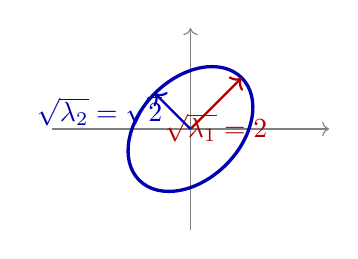
\begin{tikzpicture}[scale=0.8]
  \draw[->,gray] (-2.2,0)--(2.2,0);
  \draw[->,gray] (0,-1.6)--(0,1.6);
  \begin{scope}[rotate=45]
    \draw[blue!70!black,very thick] (0,0) ellipse (1.15 and 0.8);
    \draw[red!70!black,->,thick] (0,0)--(1.15,0) node[midway,below] {$\sqrt{\lambda_1}=2$};
    \draw[blue!70!black,->,thick] (0,0)--(0,0.8) node[midway,left] {$\sqrt{\lambda_2}=\sqrt2$};
  \end{scope}
\end{tikzpicture}
\end{center}
\end{columns}

\vspace{0.2cm}

\begin{center}
\x{Eigenvalues are squared coefficients; semi-axis lengths use square roots.}
\end{center}

\end{frame}


\begin{frame}{A Fast Negative Example}

Now consider

$$
B=\begin{pmatrix}1&2\\2&1\end{pmatrix}.
$$

\vfill

The same two directions appear:

$$
\begin{pmatrix}1\\1\end{pmatrix}
\quad\text{and}\quad
\begin{pmatrix}1\\-1\end{pmatrix}.
$$

\vfill

But the eigenvalues are:

$$
\lambda_1=3,\qquad \lambda_2=-1.
$$

\vfill

\begin{center}
\x{One negative eigenvalue: not squared length.}
\end{center}

\end{frame}


\begin{frame}[fragile]{Hyperbola from a Negative Eigenvalue}

\begin{columns}
\column{0.45\textwidth}

$$
B=\begin{pmatrix}1&2\\2&1\end{pmatrix}
$$

$$
\lambda_1=3,\quad \lambda_2=-1.
$$

\vspace{0.3cm}

One direction contributes negative squared length.

\column{0.55\textwidth}
\begin{center}
\begin{tikzpicture}[scale=0.72]
  \draw[->,gray] (-2.5,0)--(2.5,0);
  \draw[->,gray] (0,-2.0)--(0,2.0);
  \begin{scope}[rotate=45]
    \draw[blue!70!black,very thick,domain=-1.15:1.15,smooth,variable=\t]
      plot ({sinh(\t)}, {cosh(\t)})
      plot ({sinh(\t)}, {-cosh(\t)});
    \draw[gray,dashed] (-1.8,-1.8)--(1.8,1.8);
    \draw[gray,dashed] (-1.8,1.8)--(1.8,-1.8);
  \end{scope}
\end{tikzpicture}
\end{center}
\end{columns}

\vfill

\begin{center}
\x{A negative eigenvalue produces hyperbola-type geometry.}
\end{center}

\end{frame}


\begin{frame}{Eigenvalue Criterion}

\begin{thm}[Eigenvalue Criterion]
Let $A$ be a real symmetric matrix.

\begin{itemize}
\item $A$ is positive definite iff all eigenvalues are positive.
\item $A$ is positive semidefinite iff all eigenvalues are nonnegative.
\item $A$ is indefinite if it has both positive and negative eigenvalues.
\end{itemize}
\end{thm}

\vfill

\begin{center}
\x{This is the fastest conceptual test.}
\end{center}

\end{frame}


\begin{frame}{Why This Criterion Works}

From the real symmetric spectral theorem:

$$
A=\Omega\Lambda\Omega^T,
\qquad
\Omega^T\Omega=I.
$$

\vfill

Then:

$$
x^TAx
=x^T\Omega\Lambda\Omega^Tx.
$$

\vfill

Set:

$$
y=\Omega^Tx.
$$

\vfill

So:

$$
x^TAx=y^T\Lambda y.
$$

\end{frame}


\begin{frame}{Diagonal Form Shows the Signs}

If

$$
\Lambda=
\begin{pmatrix}
\lambda_1&&\\
&\lambda_2&\\
&&\ddots
\end{pmatrix},
\qquad
y=
\begin{pmatrix}
y_1\\y_2\\\vdots
\end{pmatrix},
$$

then:

$$
y^T\Lambda y
=\lambda_1y_1^2+\lambda_2y_2^2+\cdots.
$$

\vfill

\begin{center}
\x{The signs of the eigenvalues control the signs of $x^TAx$.}
\end{center}

\end{frame}


\begin{frame}{Eigenvalue Criterion Summary}

\begin{center}
\renewcommand{\arraystretch}{1.25}
\begin{tabular}{c|c|c}
\textbf{Eigenvalues} & \textbf{Form} & \textbf{Shape}\\
\hline
all $>0$ & positive except $0$ & ellipse\\
all $\ge0$ & never negative & degenerate\\
mixed signs & both signs & hyperbola
\end{tabular}
\end{center}

\vfill

\begin{center}
\x{The spectral theorem turns positivity into a diagonal sign check.}
\end{center}

\end{frame}


% ═══════════════════════════════════════
% §5 SPECTRAL FACTORIZATION
% ADR: Return to the opening question A=M^T M, but explicitly mark this
% as the spectral factorization route. A second route by diagonal
% cross-filling comes later, so this is not the only factorization story.
% ═══════════════════════════════════════
\section{Spectral Factorization}

\begin{frame}{Return to the Opening Question}

We asked:

$$
\boxed{\text{When can }A=M^TM?}
$$

\vfill

We already know one direction:

$$
A=M^TM
\quad\Longrightarrow\quad
x^TAx=\|Mx\|^2\ge0.
$$

\vfill

So:

$$
A=M^TM\quad\Longrightarrow\quad A\text{ is positive semidefinite.}
$$

\end{frame}


\begin{frame}{The Converse Should Use Eigenvalues}

Suppose $A$ is positive semidefinite.

\vfill

By the eigenvalue criterion:

$$
A=\Omega\Lambda\Omega^T,
\qquad
\lambda_i\ge0.
$$

\vfill

Since the eigenvalues are nonnegative, we can take square roots:

$$
\sqrt{\Lambda}=
\begin{pmatrix}
\sqrt{\lambda_1}&&\\
&\sqrt{\lambda_2}&\\
&&\ddots
\end{pmatrix}.
$$

\vfill

\begin{center}
\x{This is exactly where positive semidefinite matters.}
\end{center}

\end{frame}


\begin{frame}{Build the Factor}

Since

$$
\Lambda=\sqrt{\Lambda}\sqrt{\Lambda},
$$

we get:

$$
A=\Omega\sqrt{\Lambda}\sqrt{\Lambda}\Omega^T.
$$

\vfill

Now regroup:

$$
A=(\sqrt{\Lambda}\Omega^T)^T(\sqrt{\Lambda}\Omega^T).
$$

\vfill

Therefore take:

$$
\boxed{M=\sqrt{\Lambda}\Omega^T.}
$$

\end{frame}


\begin{frame}{Spectral Factorization Criterion}

\begin{thm}[Spectral Factorization Criterion]
For a real symmetric matrix $A$,

$$
\boxed{A=M^TM\text{ for some }M}
$$

if and only if

$$
\boxed{A\text{ is positive semidefinite}.}
$$
\end{thm}

\vfill

If $M$ has linearly independent columns, then:

$$
x^TM^TMx=\|Mx\|^2>0
\qquad(x\ne0),
$$

so $M^TM$ is positive definite.

\end{frame}


\begin{frame}{There Will Be a Second Factorization}

\[
\scriptsize
\underbrace{A=\Omega\Lambda\Omega^T}_{\text{spectral route}}
\quad\Longrightarrow\quad
\underbrace{A=M^TM}_{\text{factorization by eigenvalues}}.
\]

\vfill

\[
\scriptsize
\underbrace{A=P_1+P_2+\cdots+P_r}_{\text{diagonal cross-filling route}}
\quad\Longrightarrow\quad
\underbrace{A=NN^T}_{\text{factorization by cross-filled columns}}.
\]

\vfill

\begin{center}
\x{So the eigenvalue construction is one factorization, not the end of the story.}
\end{center}

\end{frame}


\begin{frame}{Concrete Positive Example}

For

$$
A=\begin{pmatrix}3&1\\1&3\end{pmatrix},
$$

we have eigenvalues $4$ and $2$.

\vfill

So:

$$
\sqrt{\Lambda}=
\begin{pmatrix}
2&0\\
0&\sqrt2
\end{pmatrix}.
$$

\vfill

With orthogonal eigenvector matrix $\Omega$:

$$
\boxed{A=(\sqrt{\Lambda}\Omega^T)^T(\sqrt{\Lambda}\Omega^T).}
$$

\end{frame}


\begin{frame}{What We Have So Far}

We now have two criteria:

\vfill

\begin{center}
\renewcommand{\arraystretch}{1.35}
\begin{tabular}{c|c}
\textbf{Criterion} & \textbf{Test}\\
\hline
Eigenvalues & all $\lambda_i\ge0$ or $>0$\\
Factorization & $A=M^TM$
\end{tabular}
\end{center}

\vfill

\begin{center}
\x{Next: a cross-filling criterion that does not start by finding eigenvalues.}
\end{center}

\end{frame}


% ═══════════════════════════════════════
% §6 DIAGONAL CROSS-FILLING CRITERION
% ADR: State the cross-filling criterion first. Cauchy is introduced only
% as the proof engine for the two PSD facts needed by the criterion.
% ═══════════════════════════════════════
\section{Checking Semipositivity by Diagonal Cross-Filling}


\begin{frame}[shrink=8]{Cross-Filling Criterion: Two Directions}

\[
\scriptsize
\underbrace{\text{positive-pivot cross-filling succeeds}}_{\substack{\text{every used pivot }p_k>0\\\text{zero rows/columns may be skipped}}}
\quad\Longrightarrow\quad
\underbrace{A=MM^T}_{\text{stack cross-filled columns}}
\quad\Longrightarrow\quad
\underbrace{A\succeq0}_{\text{easy direction}}.
\]

\vfill

\[
\scriptsize
\underbrace{A\succeq0}_{\text{hard direction}}
\quad\Longrightarrow\quad
\underbrace{\text{cross-filling can proceed legally}}_{\text{needs three modules}}.
\]

\vfill

\[
\scriptsize
\boxed{
\begin{array}{c}
\text{The easy direction constructs }MM^T.\\[0.2em]
\text{The hard direction proves PSD matrices never get stuck.}
\end{array}}
\]

\end{frame}


\begin{frame}[shrink=8]{Easy Direction: Positive Pivots Build Columns}

\[
\scriptsize
\underbrace{
\begin{pmatrix}
b_1\\ b_2\\ b_3
\end{pmatrix}}_{\text{pivot column}}
\qquad
\underbrace{b_2>0}_{\text{positive pivot}}
\qquad
\Longrightarrow
\qquad
\underbrace{m=\frac1{\sqrt{b_2}}
\begin{pmatrix}
b_1\\ b_2\\ b_3
\end{pmatrix}}_{\text{cross-filled column}}.
\]

\vfill

\[
\scriptsize
\underbrace{mm^T}_{\text{one PSD piece}}
=
\underbrace{\frac1{b_2}
\begin{pmatrix}b_1\\ b_2\\ b_3\end{pmatrix}
\begin{pmatrix}b_1&b_2&b_3\end{pmatrix}}_{P}.
\]

\vfill

\begin{center}
\x{The positive pivot is required because the column uses $\sqrt{b_2}$.}
\end{center}

\end{frame}


\begin{frame}[shrink=8]{Easy Direction: Stack All Cross-Filled Columns}

\[
\scriptsize
\underbrace{A}_{\text{after successful cross-filling}}
=
\underbrace{m_1m_1^T+m_2m_2^T+\cdots+m_rm_r^T}_{\text{rank-one PSD pieces}}.
\]

\vfill

\[
\scriptsize
\underbrace{
M=
\begin{pmatrix}
|&|&&|\\
m_1&m_2&\cdots&m_r\\
|&|&&|
\end{pmatrix}}_{\text{stack the cross-filled columns}}
\qquad\Longrightarrow\qquad
\underbrace{A=MM^T}_{\text{factorization}}.
\]

\vfill

\[
\scriptsize
\underbrace{x^TAx}_{\text{test vector}}
=
\underbrace{x^TMM^Tx}_{\text{factorized form}}
=
\underbrace{\|M^Tx\|^2}_{\ge0}.
\]

\end{frame}


\begin{frame}[shrink=8]{Hard Direction: Three Modules}

\[
\scriptsize
\underbrace{A\succeq0}_{\text{input assumption}}
\quad\Longrightarrow\quad
\begin{cases}
\underbrace{a_{ii}=e_i^TAe_i\ge0}_{\text{Module 1: no negative diagonal}},\\[0.5em]
\underbrace{a_{ii}=0\Rightarrow \text{row }i\text{ and column }i\text{ are zero}}_{\text{Module 2: zero pivot is harmless}},\\[0.5em]
\underbrace{a_{ii}>0\Rightarrow A=P+R,\quad P\succeq0,\quad R\succeq0}_{\text{Module 3: positive pivot keeps induction alive}}.
\end{cases}
\]

\vfill

\[
\scriptsize
\boxed{
\text{zero pivot }\Rightarrow\text{ skip}
\qquad
\text{positive pivot }\Rightarrow\text{ cross-fill and continue}.}
\]

\end{frame}


\begin{frame}{One Diagonal Cross-Fill Step}

Use the second diagonal entry as the visible pivot:

$$
a_{22}=e_2^TAe_2>0.
$$

\vfill

\[
\underbrace{
\begin{pmatrix}
a_{11}&\bl{a_{12}}&a_{13}\\
\bl{a_{21}}&\rd{a_{22}}&\bl{a_{23}}\\
a_{31}&\bl{a_{32}}&a_{33}
\end{pmatrix}}_{A}
=
\underbrace{
\begin{pmatrix}
p_{11}&\bl{a_{12}}&p_{13}\\
\bl{a_{21}}&\rd{a_{22}}&\bl{a_{23}}\\
p_{31}&\bl{a_{32}}&p_{33}
\end{pmatrix}}_{P}
+
\underbrace{
\begin{pmatrix}
r_{11}&0&r_{13}\\
0&\rd{0}&0\\
r_{31}&0&r_{33}
\end{pmatrix}}_{R=A-P}.
\]

\vfill

\begin{center}
\x{Diagonal cross-filling means: honestly write the two matrices $P$ and $R$.}
\end{center}

\end{frame}


\begin{frame}{Entries of the Rank-One Piece}

At the pivot $a_{22}$, write the pivot column entries as

$$
b_1=a_{12},\qquad b_2=a_{22},\qquad b_3=a_{32}.
$$

\vfill

\[
\underbrace{
\begin{pmatrix}
\dfrac{b_1b_1}{b_2}&b_1&\dfrac{b_1b_3}{b_2}\\[0.8em]
b_1&\rd{b_2}&b_3\\[0.4em]
\dfrac{b_3b_1}{b_2}&b_3&\dfrac{b_3b_3}{b_2}
\end{pmatrix}}_{P}
\]

\begin{center}
\x{This is the honest entrywise matrix display of the rank-one piece.}
\end{center}

\end{frame}



\begin{frame}[shrink=8]{Inner Product Meaning of the Entries}

\[
\scriptsize
\underbrace{
\begin{pmatrix}
\dfrac{\langle \bl{e_1},\rd{e_2}\rangle_A\langle \rd{e_2},\bl{e_1}\rangle_A}{\langle \rd{e_2},\rd{e_2}\rangle_A}
&
\langle \bl{e_1},\rd{e_2}\rangle_A
&
\dfrac{\langle \bl{e_1},\rd{e_2}\rangle_A\langle \rd{e_2},\gn{e_3}\rangle_A}{\langle \rd{e_2},\rd{e_2}\rangle_A}
\\[1.0em]
\langle \rd{e_2},\bl{e_1}\rangle_A
&
\langle \rd{e_2},\rd{e_2}\rangle_A
&
\langle \rd{e_2},\gn{e_3}\rangle_A
\\[0.6em]
\dfrac{\langle \gn{e_3},\rd{e_2}\rangle_A\langle \rd{e_2},\bl{e_1}\rangle_A}{\langle \rd{e_2},\rd{e_2}\rangle_A}
&
\langle \gn{e_3},\rd{e_2}\rangle_A
&
\dfrac{\langle \gn{e_3},\rd{e_2}\rangle_A\langle \rd{e_2},\gn{e_3}\rangle_A}{\langle \rd{e_2},\rd{e_2}\rangle_A}
\end{pmatrix}}_{P\text{ written entrywise from colored basis vectors}}
\]

\vfill

\[
\scriptsize
\underbrace{\bl{e_1}}_{\text{first row/column}}
\qquad
\underbrace{\rd{e_2}}_{\text{pivot direction}}
\qquad
\underbrace{\gn{e_3}}_{\text{third row/column}}.
\]

\vfill

\begin{center}
\x{Only the vectors are colored; each inner product remains one object.}
\end{center}

\end{frame}


\begin{frame}{Module 1: No Negative Diagonal}

\[
\scriptsize
\underbrace{A\succeq0}_{\text{PSD assumption}}
\qquad\Longrightarrow\qquad
\underbrace{a_{ii}=e_i^TAe_i\ge0}_{\text{test vector }e_i}.
\]

\vfill

\[
\scriptsize
\boxed{
\underbrace{a_{ii}<0}_{\text{negative diagonal appears}}
\quad\Longrightarrow\quad
\underbrace{A\not\succeq0}_{\text{stop cross-filling test}}.
}
\]

\vfill

\begin{center}
\x{This explains why negative pivots immediately fail the PSD test.}
\end{center}

\end{frame}



\begin{frame}[shrink=8]{Lemma: Cauchy Is the Tool for Continuation}

\[
\scriptsize
\underbrace{A\succeq0}_{\text{PSD form}}
\qquad\Longrightarrow\qquad
\underbrace{\langle x,y\rangle_A^2
\le
\langle x,x\rangle_A\langle y,y\rangle_A}_{\text{Cauchy lemma}}.
\]

\vfill

\begin{prop}[Cauchy Inequality for PSD Forms]
If $A$ is positive semidefinite and $\langle x,y\rangle_A=x^TAy$, then
$$
\langle x,y\rangle_A^2
\le
\langle x,x\rangle_A\langle y,y\rangle_A.
$$
\end{prop}

\vfill

\[
\scriptsize
\boxed{
\begin{array}{ccl}
\text{Use 1} &:& a_{ii}=0\Rightarrow \text{zero row/column},\\[0.2em]
\text{Use 2} &:& a_{ii}>0\Rightarrow R=A-P\succeq0.
\end{array}}
\]

\vfill

\begin{center}
\x{The purpose of Cauchy is to keep cross-filling alive.}
\end{center}

\end{frame}


\begin{frame}{Module 2: Zero Diagonal Means Zero Row}

\begin{prop}[Zero Diagonal Lemma]
If $A\succeq0$ and

$$
a_{ii}=e_i^TAe_i=0,
$$

then the whole $i$-th row and the whole $i$-th column are zero.
\end{prop}

\vfill

For any $j$, Cauchy gives:

$$
a_{ij}^2
=\langle e_i,e_j\rangle_A^2
\le
\langle e_i,e_i\rangle_A\langle e_j,e_j\rangle_A
=0\cdot a_{jj}=0.
$$

\vfill

So $a_{ij}=0$ for every $j$.

\end{frame}


\begin{frame}{Module 2 Meaning: Skip Zero Rows}

If $A\succeq0$ and a diagonal entry is zero:

$$
a_{ii}=0,
$$

then the whole row and column are already zero.

\vfill

\begin{center}
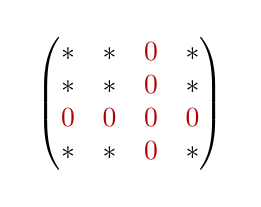
\begin{tikzpicture}[scale=0.85]
  \node at (0,0) {$
  \begin{pmatrix}
  *&*&\rd{0}&*\\
  *&*&\rd{0}&*\\
  \rd{0}&\rd{0}&\rd{0}&\rd{0}\\
  *&*&\rd{0}&*
  \end{pmatrix}$};
\end{tikzpicture}
\end{center}

\vfill

\begin{center}
\x{There is no need to choose this as a pivot. Skip it.}
\end{center}

\end{frame}


\begin{frame}{Module 3: Positive Pivot Splits PSD}

Now assume the diagonal pivot is positive:

$$
a_{ii}=e_i^TAe_i>0.
$$

\vfill

\begin{prop}[Positive Pivot Step]
If $A\succeq0$ and $a_{ii}>0$, then diagonal cross-filling gives

$$
A=P+R,\qquad P\succeq0,\qquad R\succeq0.
$$

\end{prop}

\vfill

\begin{center}
\x{Now prove it by looking at the actual entries of $P$ and $R$.}
\end{center}

\end{frame}



\begin{frame}[shrink=8]{Module 3 Setup: Write $A$ as Inner Products}

\[
\scriptsize
\underbrace{\langle \rd{e_2},\rd{e_2}\rangle_A>0}_{\text{positive pivot}}
\]

\vfill

\[
\tiny
\underbrace{
\begin{pmatrix}
\langle \bl{e_1},\bl{e_1}\rangle_A&\langle \bl{e_1},\rd{e_2}\rangle_A&\langle \bl{e_1},\gn{e_3}\rangle_A\\[0.35em]
\langle \rd{e_2},\bl{e_1}\rangle_A&\langle \rd{e_2},\rd{e_2}\rangle_A&\langle \rd{e_2},\gn{e_3}\rangle_A\\[0.35em]
\langle \gn{e_3},\bl{e_1}\rangle_A&\langle \gn{e_3},\rd{e_2}\rangle_A&\langle \gn{e_3},\gn{e_3}\rangle_A
\end{pmatrix}}_{A\text{ as an inner product table}}
\]

\vfill

\begin{center}
\x{Only the basis vectors are colored. Each inner product stays one object.}
\end{center}

\end{frame}


\begin{frame}[shrink=8]{Module 3: The Cross-Filled Piece $P$}

\[
\tiny
\underbrace{
\begin{pmatrix}
\dfrac{\langle \bl{e_1},\rd{e_2}\rangle_A\langle \rd{e_2},\bl{e_1}\rangle_A}{\langle \rd{e_2},\rd{e_2}\rangle_A}
&
\langle \bl{e_1},\rd{e_2}\rangle_A
&
\dfrac{\langle \bl{e_1},\rd{e_2}\rangle_A\langle \rd{e_2},\gn{e_3}\rangle_A}{\langle \rd{e_2},\rd{e_2}\rangle_A}
\\[1.05em]
\langle \rd{e_2},\bl{e_1}\rangle_A
&
\langle \rd{e_2},\rd{e_2}\rangle_A
&
\langle \rd{e_2},\gn{e_3}\rangle_A
\\[0.6em]
\dfrac{\langle \gn{e_3},\rd{e_2}\rangle_A\langle \rd{e_2},\bl{e_1}\rangle_A}{\langle \rd{e_2},\rd{e_2}\rangle_A}
&
\langle \gn{e_3},\rd{e_2}\rangle_A
&
\dfrac{\langle \gn{e_3},\rd{e_2}\rangle_A\langle \rd{e_2},\gn{e_3}\rangle_A}{\langle \rd{e_2},\rd{e_2}\rangle_A}
\end{pmatrix}}_{P}
\]

\vfill

\[
\scriptsize
\underbrace{P=mm^T}_{\text{PSD piece}},
\qquad
\underbrace{m=\frac1{\sqrt{\langle \rd{e_2},\rd{e_2}\rangle_A}}
\begin{pmatrix}
\langle \bl{e_1},\rd{e_2}\rangle_A\\[0.2em]
\langle \rd{e_2},\rd{e_2}\rangle_A\\[0.2em]
\langle \gn{e_3},\rd{e_2}\rangle_A
\end{pmatrix}}_{\text{positive pivot gives the square root}}.
\]

\end{frame}


\begin{frame}[shrink=8]{Module 3: The Remainder $R=A-P$}

\[
\tiny
\underbrace{R}_{A-P}
=
\underbrace{
\begin{pmatrix}
\langle \bl{e_1},\bl{e_1}\rangle_A-\dfrac{\langle \bl{e_1},\rd{e_2}\rangle_A\langle \rd{e_2},\bl{e_1}\rangle_A}{\langle \rd{e_2},\rd{e_2}\rangle_A}
&0&
\langle \bl{e_1},\gn{e_3}\rangle_A-\dfrac{\langle \bl{e_1},\rd{e_2}\rangle_A\langle \rd{e_2},\gn{e_3}\rangle_A}{\langle \rd{e_2},\rd{e_2}\rangle_A}
\\[1.25em]
0&0&0
\\[0.6em]
\langle \gn{e_3},\bl{e_1}\rangle_A-\dfrac{\langle \gn{e_3},\rd{e_2}\rangle_A\langle \rd{e_2},\bl{e_1}\rangle_A}{\langle \rd{e_2},\rd{e_2}\rangle_A}
&0&
\langle \gn{e_3},\gn{e_3}\rangle_A-\dfrac{\langle \gn{e_3},\rd{e_2}\rangle_A\langle \rd{e_2},\gn{e_3}\rangle_A}{\langle \rd{e_2},\rd{e_2}\rangle_A}
\end{pmatrix}}_{\text{entrywise remainder}}
\]

\vfill

\begin{center}
\x{The pivot row and pivot column are zero; only the remaining block must stay PSD.}
\end{center}

\end{frame}


\begin{frame}[shrink=8]{Module 3: Test the Remainder}

\[
\scriptsize
\underbrace{v}_{\text{testing vector}}
=
\underbrace{x_1\bl{e_1}+x_2\rd{e_2}+x_3\gn{e_3}}_{\text{any vector}}.
\]

\vfill

\[
\scriptsize
\underbrace{v^TRv}_{\text{test }R\text{ on both sides}}
=
\underbrace{v^T(A-P)v}_{R=A-P}
=
\underbrace{\langle v,v\rangle_A}_{v^TAv}
-
\underbrace{\frac{\langle v,\rd{e_2}\rangle_A^2}{\langle \rd{e_2},\rd{e_2}\rangle_A}}_{v^TPv}.
\]

\vfill

\[
\scriptsize
\underbrace{\langle v,\rd{e_2}\rangle_A^2}_{\text{Cauchy numerator}}
\le
\underbrace{\langle v,v\rangle_A\langle \rd{e_2},\rd{e_2}\rangle_A}_{\text{Cauchy denominator clears}}
\quad\Longrightarrow\quad
\boxed{v^TRv\ge0.}
\]

\vfill

\begin{center}
\x{Cauchy is exactly the reason the remainder remains positive semidefinite.}
\end{center}

\end{frame}


\begin{frame}{Cross-Filling Criterion So Far}

For $A\succeq0$:

\vfill

\begin{center}
\renewcommand{\arraystretch}{1.35}
\begin{tabular}{c|c}
\textbf{Diagonal pivot} & \textbf{What happens}\\
\hline
$a_{ii}<0$ & impossible\\
$a_{ii}=0$ & row/column must be zero; skip it\\
$a_{ii}>0$ & cross-fill: $A=P+(A-P)$ with both PSD
\end{tabular}
\end{center}

\vfill

\begin{center}
\x{This is the diagonal cross-filling behavior we wanted.}
\end{center}

\end{frame}


\begin{frame}{Proof of Cauchy: Geometric Memory}

\begin{prop}[Cauchy Inequality for PSD Forms]
If $A\succeq0$ and $\langle x,y\rangle_A=x^TAy$, then
$$
\boxed{\langle x,y\rangle_A^2
\le
\langle x,x\rangle_A\langle y,y\rangle_A.}
$$
\end{prop}

\vfill

\[
\scriptsize
\underbrace{A=I}_{\text{ordinary dot product}}
\qquad\Longrightarrow\qquad
\underbrace{(x^Ty)^2\le (x^Tx)(y^Ty)}_{\text{circle intuition only}}.
\]

\vfill

\begin{center}
\x{This page is only for geometric memory, not the proof.}
\end{center}

\vfill

\end{frame}


\begin{frame}{Cauchy: Picture}

For the ordinary dot product:

$$
(x^Ty)^2\le (x^Tx)(y^Ty).
$$

\vfill

After normalizing:

$$
\left(\frac{x}{\|x\|}\right)^T
\left(\frac{y}{\|y\|}\right)
\le 1.
$$

\vfill

\begin{center}
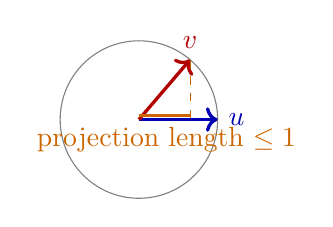
\begin{tikzpicture}[scale=1.0]
  \draw[gray] (0,0) circle (1);
  \draw[blue!70!black,very thick,->] (0,0)--(1,0) node[right] {$u$};
  \draw[red!70!black,very thick,->] (0,0)--(0.65,0.76) node[above] {$v$};
  \draw[orange!80!black,thick] (0,0.05)--(0.65,0.05);
  \draw[orange!80!black,dashed] (0.65,0.76)--(0.65,0);
  \node[orange!80!black] at (0.35,-0.25) {projection length $\le1$};
\end{tikzpicture}
\end{center}

\end{frame}


\begin{frame}{Cauchy Proof: Two Cases}

\begin{prop}[Cauchy Inequality for PSD Forms]
If $A\succeq0$, then
$$
\boxed{\langle x,y\rangle_A^2
\le
\langle x,x\rangle_A\langle y,y\rangle_A.}
$$
\end{prop}

\vfill

\begin{center}
\renewcommand{\arraystretch}{1.35}
\begin{tabular}{c|c}
\textbf{Case} & \textbf{Proof method}\\
\hline
$\langle x,x\rangle_A>0$ & build a cancellation vector $w$\\
$\langle x,x\rangle_A=0$ & use the polynomial in $t$
\end{tabular}
\end{center}

\vfill

If $\langle z,z\rangle_A=0$ for every $z$, then $A=0$ and Cauchy is trivial.

\vfill

\begin{center}
\x{So the proof is really Case 1 plus Case 2.}
\end{center}

\end{frame}


\begin{frame}{Case 1: Positive Length}

Assume the first case:

$$
\langle x,x\rangle_A>0.
$$

\vfill

Build a vector designed to cancel the $x$-component of $y$:

$$
w=\langle x,x\rangle_A\,y-\langle x,y\rangle_A\,x.
$$

\vfill

Since $A$ is positive semidefinite:

$$
0\le \langle w,w\rangle_A.
$$

\vfill

\begin{center}
\x{Now expand this one inequality.}
\end{center}

\end{frame}


\begin{frame}{Expand $\langle w,w\rangle_A$}

Let

$$
\alpha=\langle x,x\rangle_A,
\qquad
\beta=\langle x,y\rangle_A.
$$

\vfill

Then:

$$
w=\alpha y-\beta x.
$$

\vfill

So:

$$
0\le\langle w,w\rangle_A
=\langle \alpha y-\beta x,\alpha y-\beta x\rangle_A.
$$

\vfill

Using bilinearity:

$$
0\le \alpha^2\langle y,y\rangle_A-2\alpha\beta\langle x,y\rangle_A+\beta^2\langle x,x\rangle_A.
$$

\end{frame}


\begin{frame}{Finish Cauchy}

Since

$$
\beta=\langle x,y\rangle_A,
\qquad
\alpha=\langle x,x\rangle_A,
$$

the expansion becomes:

$$
0\le
\alpha^2\langle y,y\rangle_A
-2\alpha\beta^2
+\beta^2\alpha.
$$

\vfill

Combine the last two terms:

$$
0\le
\alpha^2\langle y,y\rangle_A-\alpha\beta^2.
$$

\end{frame}


\begin{frame}{Finish Cauchy (continued)}

We have:

$$
0\le
\alpha^2\langle y,y\rangle_A-\alpha\beta^2.
$$

\vfill

Divide by $\alpha=\langle x,x\rangle_A>0$:

$$
0\le \langle x,x\rangle_A\langle y,y\rangle_A-\langle x,y\rangle_A^2.
$$

\vfill

Therefore:

$$
\boxed{
\langle x,y\rangle_A^2
\le
\langle x,x\rangle_A\langle y,y\rangle_A.
}
$$

\end{frame}


\begin{frame}{Case 2: Zero Length}

What if $\langle x,x\rangle_A=0$?

\vspace{0.25cm}

For any real number $t$:

$$
0\le \langle x+ty,x+ty\rangle_A.
$$

\vspace{0.2cm}

Expanding:

$$
0\le
2t\langle x,y\rangle_A+t^2\langle y,y\rangle_A.
$$

This quadratic cannot be nonnegative for all $t$ unless:

$$
\boxed{\langle x,y\rangle_A=0.}
$$

\end{frame}


\section{Worked Cross-Filling Tests}

\begin{frame}{Test 1: Zero Diagonal Obstruction}

Consider

\[
\underbrace{
\begin{pmatrix}
1&2&-3\\
2&\rd{0}&2\\
-3&2&5
\end{pmatrix}}_{A}
\]

\vfill

If $A\succeq0$ and $a_{22}=0$, the zero diagonal lemma forces the whole second row and column to be zero.

\vfill

But here:

$$
a_{21}=2,\qquad a_{23}=2.
$$

\vfill

\begin{center}
\x{Therefore $A$ is not positive semidefinite.}
\end{center}

\end{frame}


\begin{frame}{Test 2: Negative Remainder Obstruction}

Start with

\[
\underbrace{
\begin{pmatrix}
\rd{1}&\bl{3}&\bl{2}\\
\bl{3}&5&4\\
\bl{2}&4&9
\end{pmatrix}}_{B}.
\]

\vfill

Cross-fill from the first diagonal pivot:

\[
\underbrace{
\begin{pmatrix}
1&3&2\\
3&5&4\\
2&4&9
\end{pmatrix}}_{B}
-
\underbrace{
\begin{pmatrix}
1&3&2\\
3&9&6\\
2&6&4
\end{pmatrix}}_{P}
=
\underbrace{
\begin{pmatrix}
0&0&0\\
0&\rd{-4}&-2\\
0&-2&5
\end{pmatrix}}_{R}.
\]

\vfill

\begin{center}
\x{A PSD remainder cannot have a negative diagonal entry.}
\end{center}

\end{frame}


\begin{frame}{Test 3: Positive Cross-Filling}

Now consider

\[
\underbrace{
\begin{pmatrix}
\rd{1}&\bl{3}&\bl{2}\\
\bl{3}&10&7\\
\bl{2}&7&9
\end{pmatrix}}_{A}.
\]

\vfill

First diagonal cross-fill:

\[
\underbrace{
\begin{pmatrix}
1&3&2\\
3&10&7\\
2&7&9
\end{pmatrix}}_{A}
=
\underbrace{
\begin{pmatrix}
1&3&2\\
3&9&6\\
2&6&4
\end{pmatrix}}_{P_1}
+
\underbrace{
\begin{pmatrix}
0&0&0\\
0&1&1\\
0&1&5
\end{pmatrix}}_{R_1}.
\]

\end{frame}


\begin{frame}{Test 3: Continue}

The active remainder is the lower-right block:

\[
\underbrace{
\begin{pmatrix}
0&0&0\\
0&\rd{1}&\bl{1}\\
0&\bl{1}&5
\end{pmatrix}}_{R_1}
=
\underbrace{
\begin{pmatrix}
0&0&0\\
0&1&1\\
0&1&1
\end{pmatrix}}_{P_2}
+
\underbrace{
\begin{pmatrix}
0&0&0\\
0&0&0\\
0&0&\rd{4}
\end{pmatrix}}_{R_2}.
\]

\vfill

Final pivot:

$$
R_2=
\underbrace{
\begin{pmatrix}
0&0&0\\
0&0&0\\
0&0&4
\end{pmatrix}}_{P_3}.
$$

\end{frame}


\begin{frame}{Test 3: Sum of Positive Pieces}

The whole matrix is a sum of positive rank-one pieces:

\[
\scriptsize
\begin{aligned}
\underbrace{
\begin{pmatrix}
1&3&2\\
3&10&7\\
2&7&9
\end{pmatrix}}_{A}
=
\underbrace{
\begin{pmatrix}1\\3\\2\end{pmatrix}
\begin{pmatrix}1&3&2\end{pmatrix}}_{P_1}
+
\underbrace{
\begin{pmatrix}0\\1\\1\end{pmatrix}
\begin{pmatrix}0&1&1\end{pmatrix}}_{P_2}
\\
&\quad+
\underbrace{
\begin{pmatrix}0\\0\\2\end{pmatrix}
\begin{pmatrix}0&0&2\end{pmatrix}}_{P_3}.
\end{aligned}
\]

\vfill

Therefore:

$$
x^TAx
=(x_1+3x_2+2x_3)^2+(x_2+x_3)^2+(2x_3)^2
$$

This is $>0$ for every $x\ne0$.

\end{frame}


\begin{frame}[shrink=8]{Test 3 Also Builds a Factorization}

\[
\scriptsize
\underbrace{
\begin{pmatrix}
1&3&2\\
3&10&7\\
2&7&9
\end{pmatrix}}_{A}
=
\underbrace{
\begin{pmatrix}1\\3\\2\end{pmatrix}
\begin{pmatrix}1&3&2\end{pmatrix}}_{m_1m_1^T}
+
\underbrace{
\begin{pmatrix}0\\1\\1\end{pmatrix}
\begin{pmatrix}0&1&1\end{pmatrix}}_{m_2m_2^T}
+
\underbrace{
\begin{pmatrix}0\\0\\2\end{pmatrix}
\begin{pmatrix}0&0&2\end{pmatrix}}_{m_3m_3^T}.
\]

\vfill

\[
\scriptsize
\underbrace{
M=
\begin{pmatrix}
|&|&|\\
m_1&m_2&m_3\\
|&|&|
\end{pmatrix}
=
\begin{pmatrix}
1&0&0\\
3&1&0\\
2&1&2
\end{pmatrix}}_{\text{stack the cross-filled columns}}
\qquad\Longrightarrow\qquad
\boxed{A=MM^T.}
\]

\vfill

\begin{center}
\x{Cross-filling is both a test and a constructive factorization.}
\end{center}

\end{frame}


\begin{frame}{Cross-Filling Criterion}

For a real symmetric matrix:

\vfill

\begin{center}
\small
\renewcommand{\arraystretch}{1.25}
\begin{tabular}{c|c}
\textbf{Cross-filling behavior} & \textbf{Conclusion}\\
\hline
positive pivots until zero remainder & positive definite\\
positive pivots + zero rows/columns & positive semidefinite\\
zero diagonal but nonzero row & not PSD\\
negative diagonal in remainder & not PSD
\end{tabular}
\end{center}

\vfill

\begin{center}
\x{This is the computational test from diagonal cross-filling.}
\end{center}

\end{frame}


\section{Connection to Determinants}

\begin{frame}{What the Literature Says}

Many textbooks do not say ``cross-filling.''

\vfill

They usually say:

\[
\boxed{
\begin{array}{c}
\text{positive definite}\\
\Longleftrightarrow\\
\text{certain principal determinants are positive}
\end{array}}
\]

\vfill

For example, in the no-row-swap diagonal order:

$$
\det A_1>0,\qquad \det A_2>0,\qquad \cdots,\qquad \det A_n>0.
$$

\vfill

\begin{center}
\x{This is Sylvester's determinant criterion.}
\end{center}

\end{frame}


\begin{frame}{Principal Determinants}

For a $3\times3$ matrix, leading principal determinants are:

\[
\scriptsize
\underbrace{
\begin{pmatrix}
\rd{a_{11}}&*&*\\
*&*&*\\
*&*&*
\end{pmatrix}}_{A_1}
\quad
\underbrace{
\begin{pmatrix}
\rd{a_{11}}&\rd{a_{12}}&*\\
\rd{a_{21}}&\rd{a_{22}}&*\\
*&*&*
\end{pmatrix}}_{A_2}
\quad
\underbrace{
\begin{pmatrix}
\rd{a_{11}}&\rd{a_{12}}&\rd{a_{13}}\\
\rd{a_{21}}&\rd{a_{22}}&\rd{a_{23}}\\
\rd{a_{31}}&\rd{a_{32}}&\rd{a_{33}}
\end{pmatrix}}_{A_3=A}.
\]

\vfill

The literature checks:

$$
\det A_1,\qquad \det A_2,\qquad \det A_3.
$$

\end{frame}


\begin{frame}{Our Dictionary: Determinant = Product of Pivots}

Diagonal cross-filling produces pivots:

$$
d_1,\ d_2,\ \ldots,\ d_n.
$$

\vfill

From our determinant lecture:

$$
\boxed{
\det A_k=d_1d_2\cdots d_k.
}
$$

\vfill

So the next pivot is the ratio:

$$
\boxed{
d_k=\frac{\det A_k}{\det A_{k-1}}.
}
$$

\vfill

\begin{center}
\x{Principal determinants are just cumulative products of cross-filling pivots.}
\end{center}

\end{frame}


\begin{frame}{Positive Definite: Same Test, Different Language}

Cross-filling says:

$$
d_1>0,\qquad d_2>0,\qquad \cdots,\qquad d_n>0.
$$

\vfill

Determinants say:

$$
\det A_1>0,\qquad \det A_2>0,\qquad \cdots,\qquad \det A_n>0.
$$

\vfill

They are equivalent because:

$$
\det A_k=d_1d_2\cdots d_k.
$$

\vfill

\begin{center}
\x{Same information: determinant criterion hides the pivots inside products.}
\end{center}

\end{frame}


\begin{frame}[shrink=5]{Why This Breaks for Semidefinite}

Leading determinants only see products:

$$
d_1=0
\quad\Longrightarrow\quad
\det A_1=\det A_2=\cdots=0
$$

even if some hidden direction is negative.

\vfill

\[
\underbrace{
\begin{pmatrix}
\rd{0}&0&0\\
0&1&0\\
0&0&\rd{-1}
\end{pmatrix}}_{B}
\]

\vspace{0.1cm}

Here $B$ is not PSD, but:

$$
\det B_1=0,\qquad \det B_2=0,\qquad \det B_3=0.
$$

\begin{center}
\x{Leading determinant tests cannot certify semidefinite matrices.}
\end{center}

\end{frame}


\begin{frame}{Semidefinite: Why Literature Becomes Heavier}

For positive semidefinite matrices, zero pivots can appear.

\vfill

Then leading determinants alone are not enough.  Textbooks usually say:

$$
\boxed{\text{all principal minors must be nonnegative}.}
$$

\vfill

That means many determinants, even in $3\times3$:

\[
\small
\begin{array}{c}
\det A_{\{1\}},\quad \det A_{\{2\}},\quad \det A_{\{3\}},\\[0.2em]
\det A_{\{1,2\}},\quad \det A_{\{1,3\}},\quad \det A_{\{2,3\}},\\[0.2em]
\det A_{\{1,2,3\}}.
\end{array}
\]

\vfill

\begin{center}
\x{Our zero-row rule replaces this determinant explosion with structure.}
\end{center}

\end{frame}


\begin{frame}{Complexity: Determinants vs. Pivots}

For an $n\times n$ matrix, all principal minors means one determinant for every nonempty subset:

$$
\boxed{2^n-1\text{ determinants}.}
$$

\vfill

Cross-filling checks the active diagonal behavior directly:

$$
\boxed{\text{pivots }d_k\quad+\quad\text{zero row/column rule}\quad+\quad\text{remainders}.}
$$

\vfill

\begin{center}
\renewcommand{\arraystretch}{1.25}
\begin{tabular}{c|c}
\textbf{Literature PSD test} & \textbf{Cross-filling PSD test}\\
\hline
many principal determinants & pivots and remainders\\
products hide zero pivots & zero pivots are inspected\\
sign answer only & structural obstruction
\end{tabular}
\end{center}

\end{frame}


\begin{frame}{Why Cross-Filling Is Stronger}

Determinants answer only one question:

$$
\det(\text{submatrix})\quad \text{positive, zero, or negative?}
$$

\vfill

Cross-filling gives more data:

\begin{center}
\small
\renewcommand{\arraystretch}{1.15}
\begin{tabular}{c|c}
\textbf{Cross-filling data} & \textbf{Meaning}\\
\hline
pivot $d_k$ & determinant ratio\\
rank-one piece $P_k$ & squared-length component\\
remainder $R_k$ & next active problem\\
zero row/column & semidefinite degeneracy\\
negative diagonal in $R_k$ & obstruction
\end{tabular}
\end{center}

\vfill

\begin{center}
\x{Computing determinants is essentially cross-filling with less memory.}
\end{center}

\end{frame}


\section{Applications}

\begin{frame}[shrink=8]{Application 1: Square Root of a PSD Matrix}

\[
\scriptsize
\underbrace{A\succeq0}_{\text{positive semidefinite}}
\quad\Longrightarrow\quad
\underbrace{
A=
\Omega
\begin{pmatrix}
\lambda_1&&0\\
&\ddots&\\
0&&\lambda_n
\end{pmatrix}
\Omega^T}_{\substack{\text{orthogonal diagonalization}\\\lambda_i\ge0}}.
\]

\vfill

\[
\scriptsize
\underbrace{
A^{1/2}
:=
\Omega
\begin{pmatrix}
\sqrt{\lambda_1}&&0\\
&\ddots&\\
0&&\sqrt{\lambda_n}
\end{pmatrix}
\Omega^T}_{\text{define one symmetric square root}}.
\]

\vfill

\[
\scriptsize
\underbrace{A^{1/2}A^{1/2}}_{\text{multiply in the same eigenbasis}}
=
\Omega
\begin{pmatrix}
\lambda_1&&0\\
&\ddots&\\
0&&\lambda_n
\end{pmatrix}
\Omega^T
=A.
\]

\vfill

\begin{center}
\x{Matrix square roots are not unique; this defines the symmetric PSD square root.}
\end{center}

\end{frame}


\begin{frame}[shrink=8]{Application 1: Example}

\[
\scriptsize
\underbrace{
A=
\begin{pmatrix}
3&1\\
1&3
\end{pmatrix}}_{\text{PSD}}
=
\underbrace{
\Omega}_{\text{orthogonal eigenbasis}}
\underbrace{
\begin{pmatrix}
4&0\\
0&2
\end{pmatrix}}_{\Lambda}
\underbrace{\Omega^T}_{\text{eigen-coordinate rows}}.
\]

\vfill

\[
\scriptsize
\underbrace{
A^{1/2}
:=
\Omega
\begin{pmatrix}
\sqrt4&0\\
0&\sqrt2
\end{pmatrix}
\Omega^T}_{\text{replace squared axis coefficients by axis coefficients}}
=
\underbrace{
\Omega
\begin{pmatrix}
2&0\\
0&\sqrt2
\end{pmatrix}
\Omega^T}_{\text{symmetric square root}}.
\]

\vfill

\begin{center}
\x{PSD matrices allow a real symmetric square root.}
\end{center}

\end{frame}


\begin{frame}[shrink=10]{Application 2: Comparing Two Inner Products}

\[
\scriptsize
\underbrace{A=
\Omega
\begin{pmatrix}
\lambda_1&&0\\
&\ddots&\\
0&&\lambda_n
\end{pmatrix}
\Omega^T}_{\lambda_{\min}\le\lambda_i\le\lambda_{\max}}
\qquad
\underbrace{y=\Omega^Tx}_{\text{orthogonal change of coordinates}}.
\]

\vfill

\[
\scriptsize
\underbrace{x^TAx}_{\langle x,x\rangle_A}
=
\underbrace{y^T
\begin{pmatrix}
\lambda_1&&0\\
&\ddots&\\
0&&\lambda_n
\end{pmatrix}
y}_{\lambda_1y_1^2+\cdots+\lambda_ny_n^2}.
\]

\vfill

\[
\scriptsize
\underbrace{\lambda_{\min}(y_1^2+\cdots+y_n^2)}_{\lambda_{\min}\|x\|^2}
\le
\underbrace{x^TAx}_{\text{new squared length}}
\le
\underbrace{\lambda_{\max}(y_1^2+\cdots+y_n^2)}_{\lambda_{\max}\|x\|^2}.
\]

\end{frame}


\begin{frame}{Eigenvalue Bound for the Ratio}

\[
\scriptsize
\boxed{
\lambda_{\min}
\le
\underbrace{\frac{x^TAx}{x^Tx}}_{\text{ratio of new squared length to old squared length}}
\le
\lambda_{\max}
\qquad(x\ne0).
}
\]

\vfill

\begin{thm}[Eigenvalue Comparison]
If $A$ is real symmetric with smallest eigenvalue $\lambda_{\min}$ and
largest eigenvalue $\lambda_{\max}$, then every nonzero vector $x$ satisfies
$$
\boxed{
\lambda_{\min}
\le
\frac{x^TAx}{x^Tx}
\le
\lambda_{\max}.
}
$$
\end{thm}

\vfill

\begin{center}
\x{Eigenvalues measure the strongest and weakest stretching of the inner product.}
\end{center}

\end{frame}


\section*{}

\begin{frame}{Final Summary}

Complete answer:

$$
A=M^TM
\quad\Longleftrightarrow\quad
x^TAx\ge0\quad\text{for all }x.
$$

\vspace{0.05cm}

\begin{center}
\small
\renewcommand{\arraystretch}{1.12}
\begin{tabular}{c|c}
\textbf{Test} & \textbf{PSD criterion}\\
\hline
quadratic form & $x^TAx\ge0$ for all $x$\\
eigenvalues & every $\lambda_i\ge0$\\
factorization & $A=M^TM$\\
cross-filling & positive pivots + zero-row rule
\end{tabular}
\end{center}

\vfill

\begin{center}
\x{Positive definite means the same story with strict positivity.}
\end{center}

\end{frame}

\end{document}
